\documentclass[12pt,letterpaper]{article}
\usepackage[spanish]{babel}
\usepackage[right=2cm,left=3cm,top=2cm,bottom=2cm,headsep=0cm,footskip=0.5cm]{geometry}
\usepackage{graphicx}
\usepackage{subfigure}
\usepackage[utf8]{inputenc}

\title{Trading Bitcoin with Reinforcement
Learning}
\author{Jorge A. Hernández Casildo, \\Ricardo Montesinos Fernandez, 
 \\Ismael A. Prado Segovia}


\begin{document}

\maketitle
\abstract El comercio algorítmico ha existido durante décadas y, en su mayor parte, ha disfrutado de una buena
cantidad de éxitos en sus variadas formas. Tradicionalmente, la negociación algorítmica implica la
selección de reglas de negociación cuidadosamente diseñadas, optimizadas y probadas por humanos. Si
bien estas estrategias tienen la ventaja de ser sistemáticas y de operar a velocidades y frecuencias que
van más allá de los comerciantes humanos, son susceptibles a todo tipo de sesgos de selección y no
pueden adaptarse a las cambiantes condiciones del mercado. El aprendizaje de refuerzo (RL) por otro
lado, es mucho más "libre" de elegir múltiples decisiones. En RL, un "agente" simplemente busca maximizar su recompensa
en cualquier entorno dado e intenta mejorar su toma de decisiones a través de prueba y error a medida
que experimenta más escenarios. En general, RL puede descubrir acciones que los humanos normalmente no encontrarían. Como una prueba de
concepto, diseñamos e implementamos un sistema de comercio para bitcoins como prueba del algoritmo, aunque se puede implementar con otros activos.
La arquitectura del modelo consiste en maximizar las recompensas implementando Q-learning, basado en la conocida función $Q(s,a)$ que es el valor de una acción en un estado s, aprendiendo de una red neuronal perceptron multicapa con tres capas ocultas con una capa de entrada del tamaño del estado, y funciones de activación ReLu.
\\
\\
\section{Introducci\'on}

El aprendizaje de refuerzo es apropiado cuando el espacio de estado (la descripción cuantitativa del
entorno) es grande o incluso continuo. Puede ser especialmente útil cuando no es práctico obtener
etiquetas para el aprendizaje supervisado. El comercio es un buen ejemplo de esto donde las acciones
correctas no se conocen e incluso si lo fueran, sería casi imposible de aplicar a cada situación en la que
el agente tiene que actuar. RL también es apropiado cuando, como en el comercio, las acciones tienen
consecuencias a largo plazo y las recompensas pueden retrasarse. Los ingredientes esenciales para el
aprendizaje de refuerzo son estados, acciones, recompensas y una política de selección de acción. En
un problema dado, se supone que un agente debe seleccionar la mejor acción dado su estado actual.
Esta acción produce una observación del nuevo estado, así como una recompensa, y esto se repite en lo
que se conoce como un proceso de decisión de Markov, en este caso el proceso es $Q-learning$. Para que el agente aprenda el comportamiento del historico de BTC se retroalimenta la recompensa para una secuencia de estados (window) por medio de Q-learnig. Hay dos formas principales de formular el problema: basado en valores y
basado en políticas. En un enfoque basado en el valor, se estima el valor de cada estado o el par
acción- estado. La política se genera al estimar con precisión estos valores y luego seleccionar la acción
con el valor más alto. En un enfoque basado en políticas, que es nuestro método elegido, directamente
parametrizamos la política y luego encontramos los parámetros que maximizan las recompensas 
esperadas.


 \section{ Basicos de Reinforcement Learning}

EL Aprendizaje refozado (RL) es uno de los paradigmas del aprendizaje maquina y consiste en un agente que aprende a comportarse o a actuar en un ambiente estocástico y en muchas ocasiones desconocido esto es posible por una retroalimentación que tiene el agente llamada recompensa. La meta del agente es seleccionar las acciones adecuadas que maximicen las recompensas. Sin embargo siempre que el ambiente involucre factores estocásticos que afecten a la elección de acciones el agente deberá balancear su comportamiento greedy para tener mejores recompensas en un futuro. Podriamos definir los algoritmos de aprendizaje reforzado como metrodos computacionales que resuelven problemas en una secuencia de desciciones que interactúan con el ambiente, donde estas acciones pueden o no modificar el ambiente. 
\newline
%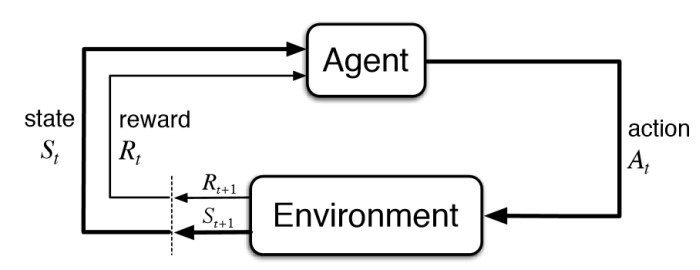
\includegraphics[height=\baselineskip]{agent.jpg}

\textbf{Proceso de Decisión de Markov}
\newline 

Los problemas que involucran una secuencia de decisiones generalmente son tratados mediante un proceso de decisión de Markov (MDP). 
Un MDP es un sistema estocásticamente dinamico definido por una tupla $< S, A, P, R, \gamma > $  donde $(S,s)$ es un espacio de estado medible, $(A,a)$, es un espacio de acción medible $( P:S \times A \times s \rightarrow R )$es una transición, $(R:S \times A)$ es una función de recompensa y gamma es una función de descuento entre [0 y 1].  Suponemos que en un tiempo t existe un stedo $S_t = s$ y el agente toma la acción $A_t = a$ entonces probabilidad del siguiente estado $S_{t+1}$ esta dada por la siguiente expresión: 
\newline \newline
$ P(s,a,s’) = P(S_{t+1} | S_t,A_t)$ 
\newline \newline
Con una recompensa dada por: 
\newline
\newline 
$R(s,a) = E[R_{t=1}|S_t,A_t]$
\newline \newline
Una vez obtenida esta retroalimentación dada por la recompensa el agente selecciona una política $(\pi: S \times A\rightarrow R)$ tal que cada estado tiene una distribución de probabilidad para cada acción, generando una ganancia especifica por política: 
\newline
\newline 
$G_t= \sum\limits_{t=0}^\infty \gamma^t R_{t+k+1}$ 
\newline
\newline 

Sin embargo ya que nuestra ganancia es estocástica el agente considera un valor esperado que también es conocido como función de estado valor 
\newline
\newline 
$V_{\pi}(s) = E_{\pi}[G_t | S_t = s]$
\newline
\newline 
Esta ecuación evalúa que tan bien actúa el agente dado un estado bajo una política, muy similarmente esta la función de acción valor 
\newline
\newline 
$q_{\pi} = \sum\limits_a \pi(a|s) \sum\limits_{s',r} p(s',R|s,a)[r + \gamma v_{\pi}(s')]$
\newline
\newline 
Una vez determinadas estas ecuaciones podemos observar una relación entre $V_{\pi}$ y $Q_{\pi}$ y esta relación esta dada por las ecuaciones de Bellman:
\newline
\newline 
{$V_{\pi}(s) = \sum\limits_{a} \pi(s,a)  \sum\limits_{s'} P[R + \gamma V_{\pi} (s')]$
\newline
\newline
$Q_{\pi}(s,a) = \sum\limits_{s'} = P[R + \gamma \sum\limits_{a'} Q_{\pi}(s',a')] $ 
\newline
\newline 
Se busca que los valores estado-acción sean maximizados y de esta manera surge uno de los mas populares algoritmos de RL y es el algoritmo de Q-learning y la idea de aplicación es bastante simple. Consiste en aplicar una estimación de incremento a la ecuación. 
\newline
\newline 
\textbf{Q-learning}
\newline
\newline 
Q-learning es un método propuesto para resolver MDP con información incompleta, a medida que el agente se mueve de un estado a un estado mas reciente, el Q-lerning considera las estimaciones de los Q pasados para el nuevo estado. 
Idealmente el ciclo de Q-learning se realiza de forma infinita, pero en la practica se realiza por el numero de episodios seleccionados donde cada episodio comienza en un estado inicial hasta alcanzar una condición objetivo como llegar a algún estado, o cierto numero de iteraciones. 
Este método también utiliza un factor $\alpha$ que es denominado parámetro del tamaño pasado y regularmente se encuentra entre $[0$ y $1]$. Este parámetro determina la importancia de los estados pasados para la predicción del futuro, y puede ser variado con cada iteración. 

En Q-learning cada estado, acción y recompensa acumulada, son guardados en una tabla donde se pueden ver todos los estados anteriores para sus futuras acciones, esta tabla es denominada Q-table. 
Esta tabla es el principal obstáculo al tratar con ambientes donde el agente tiene muchos estados o donde el ambiente cambia constantemente como una serie de tiempo, pues almacenar cada estado en la tabla puede requerir mucho espacio de memoria y tiempo al leer la tabla. 
 
\section{Definici\'on del problema }

EL problema consiste en un agente que compra y vende algun activo financieros, en este caso bitcoins, durante cierto tiempo T cuyo objetivo es maximizar las ganancias. 

Para una mejor comprensión del problema definiermos algunos aspectos fundamentales en RL aplicados a nuestro problema: 
\begin{itemize}
\item Agente: Es el encargado de realizar el Trading. 
\item Ambiente: los precios de acuerdo al tiempo T.
\item Estado: precio al momento T 
\item Acciones: son 3 las acciones que nuestro agente puede realizar y son: “Comprar, Vender y Mantenerse ”
\item Recompensas: El agente obtiene una recompensa cada vez que vende un bitcoin y esta recompensa esta relacionada con el rendimiento obtenido con esa venta. 
\end{itemize}

Al tratarse de un activo que va cambiando con el tiempo se utilzo una ventana de tiempo con el fin de crear Q-tables pequenas y mas faciles de analizar, tenuendo una ventana de 32 estados cada ventana. Los resultados de cada ventana son evaluados cadda cierto perido conocido como episodios.

Nuestro agente no modifica el ambiente pero si consideramos cada "trader" como un agente y todos los agentes juntos podrian cambiar el estado y precio del bitcoin 


\section{Experimentaci\'on y Resultados}
Se comienza a experimentar con los datos del historial de precio del Bitcoin \textit{BTC} en dolares (de un archivo CSV). Estos datos servirán para entrenar al agente del algoritmo de Q-learning. La idea es poder invertir dinero en cierto tiempo y obtener pequeñas ganancias en intervalos de tiempo cortos. \\

Iniciamos el experimento con un saldo inicial o \textit{balance}, una cantidad positiva fija de \textit{criptomonedas} y un numero de episodios, los cuales están definidos por la \textit{longitud de los datos del archivo CSV / el tamaño del episodio}. Teniendo estos datos, comenzamos a iterar en cada \textit{step}, cada step es definido como el precio del bitcon en el tiempo $t$.\\

Dentro de nuestro código nos apoyamos de la función Sigmoide para obtener un arreglo de tres valores en el siguiente orden $[BUY, SELL,  HOLD]$, luego entonces, elegimos la acción con el mayor valor de probabilidad.\\
Cada acción actualiza el \textit{balance}, el número de bitcoins adquiridos y la ganancia final. Recordemos que la idea es obtener la mayor cantidad de ganancia posible, para ello nos apoyamos en la siguiente ecuación, donde $p(t)$ es el precio del bitcoin en el tiempo $t$.
\begin{center}
$reward = bitcoins*[p(t)/p(t-1)-1]$
\end{center}
En cada iteración actualizamos el Q-table con los valores del estado actual \textbf{s}, la acción elegida \textbf{a}, la ganancia obtenida o reward \textbf{r } y el valor del siguiente estado \textbf{s'}.
Una vez actualizado el Q-table, utilizamos los valores de \textbf{s, a, r, s'} para alimentar la formula de acción valor, obtener el siguiente estado y volver a iterar dentro del episodio.\\
\\
Los resultados  finales son variables, pero en todos los casos se obtiene una ganancia. En la siguiente gráfica se observa que iniciamos con un Balance cercano a \textit{200 USD}, con muchas alzas y bajas pero con tendencia positiva, al final la ganancia es cercana a los \textit{1000 USD}.


\begin{center}
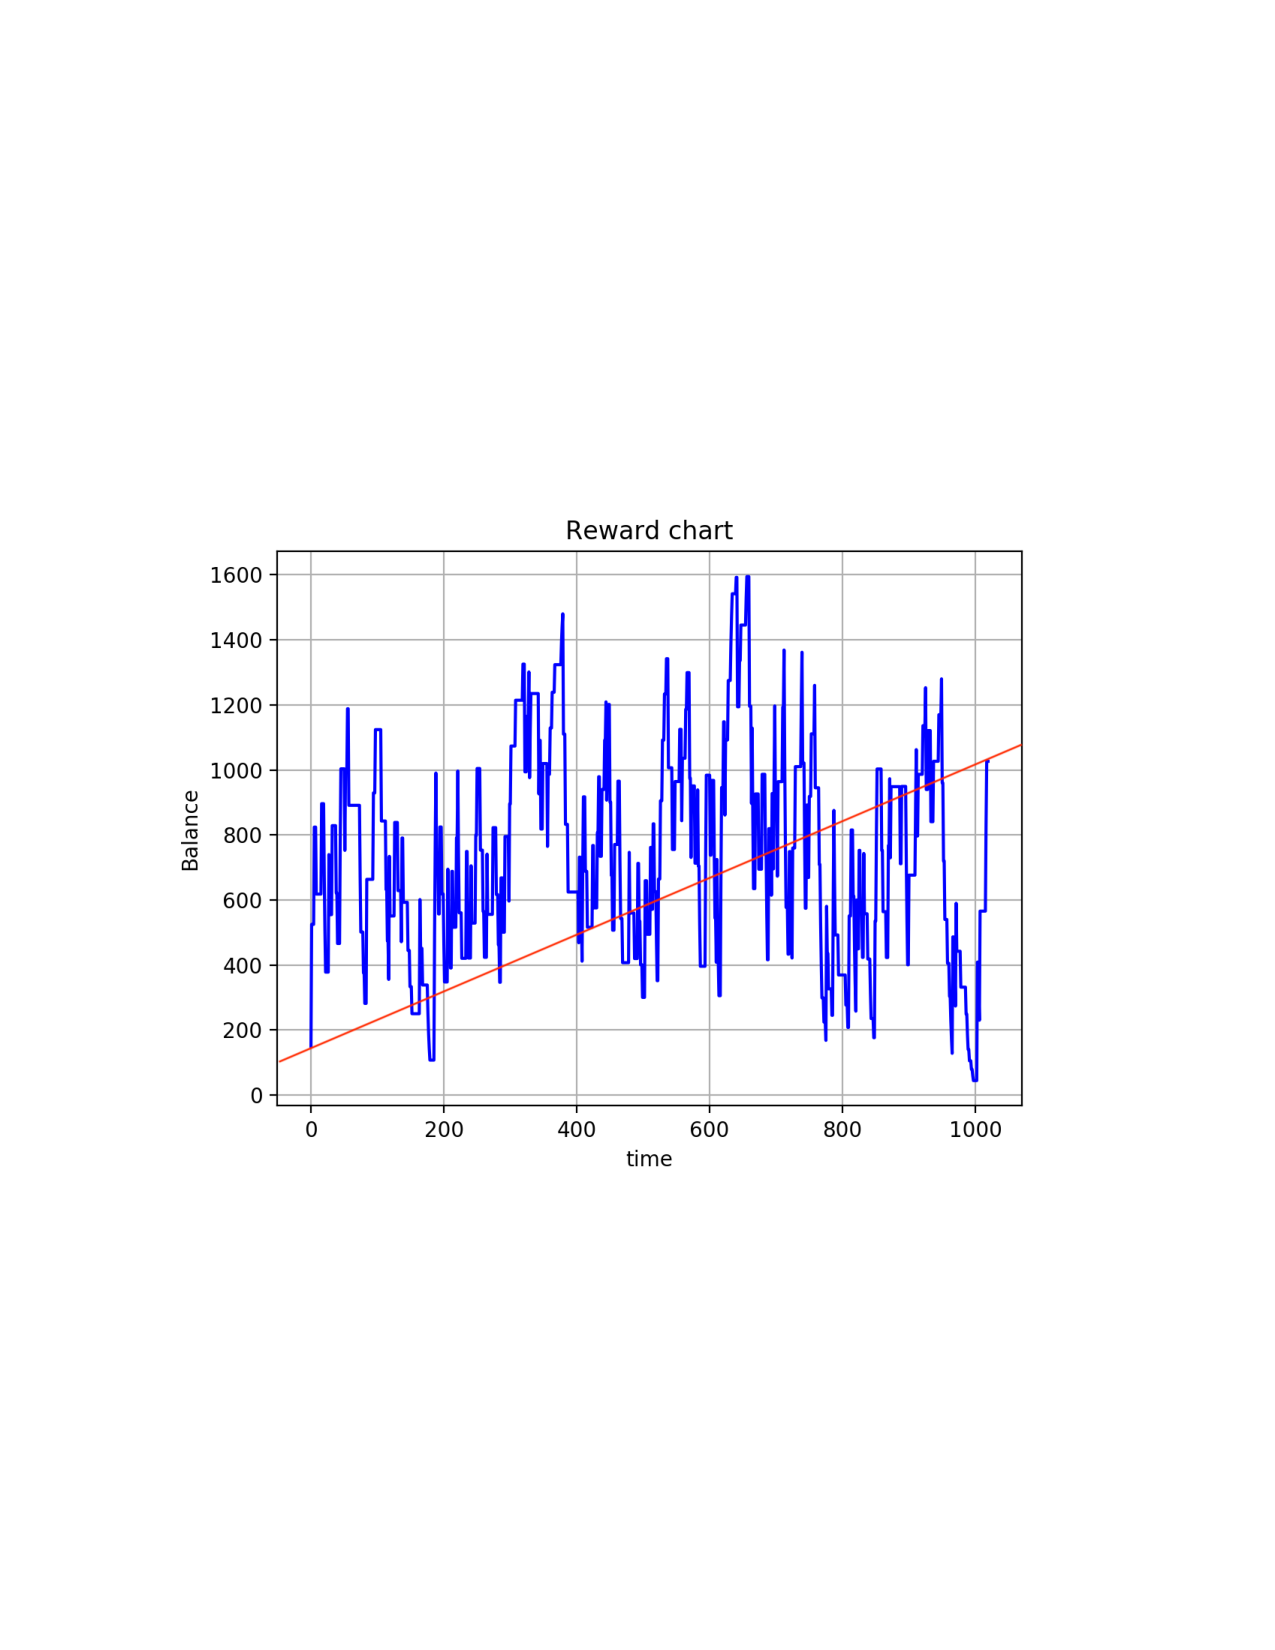
\includegraphics[width=0.8\textwidth]{rewardchart.png}
\end{center}

\section{Conclusiones} 
En este experimento se pueden obtener ganancias positivas y quizás se pueda llegar a pensar en que el algoritmo funciona, sin embargo el algoritmo de Q-learning por si solo no funciona para tratar problemas que cambian en el tiempo y cuyos estados pueden variar demasiado como el caso del bitcoin, para esto es necesario apoyarse de otras herramientas que complementen el aprendizaje reforzado como son las redes neuronales, o incluso otros métodos que no sea Q-learning.

El Q-learning es efectivo para tareas donde el ambiente no cambia y la cantidad de estados son fijos.

Por si mismo, el problema de \textit{trading} es muy complejo, y Q-learning podría no ser la via para resolver el problema de obtener la máxima ganancia mediante \textit{tradings} inteligentes.


\section{Referencias}

Trading Bitcoin with Reinforcement Learning. Introduction to Algorithmic Trading [https://launchpad.ai/blog/trading-bitcoin]\\

Sutton, R. and Barto, A.: Introduction to reinforcement learning. (2017)\\

Forecasting: Principles and Practice. Rob J Hyndman and George Athanasopoulos.


\end{document}